\chapter{Solver nonogramów}
\thispagestyle{chapterBeginStyle}

    W tym rozdziale opisany jest rozwój solvera. Przedstawione są kolejne wersje solverów, wraz z
opisem ich działania. Zbadany został wpływ zastosowanych heurystyk na wydajność w rozwiązywaniu 
wybranych łamigłówek. Podany został także schemat dla łamigłówek znajdujących się w aplikacji.



\section{Wersje solverów}


\subsection{Solver całościowy}
    Solver całościowy jest najprostszym z solverów implementowanych w toku pisania aplikacji. Jego
implementacja opiera się na założeniu, że obrazek ukryty w łamigłówce jest ciągiem pustych i pełnych
pikseli. Solver sprawdza wszystkie możliwe kombinacje pól, aż do wykrycia rozwiązania, bądź stwierdzenia
jego braku. Wskazówki umieszczone obok planszy służą jedynie do walidacji rozwiązania i nie są
wykorzystywane w trakcie rozwiązywania nonogramu.

\begin{figure}[!htb]
    \centering
    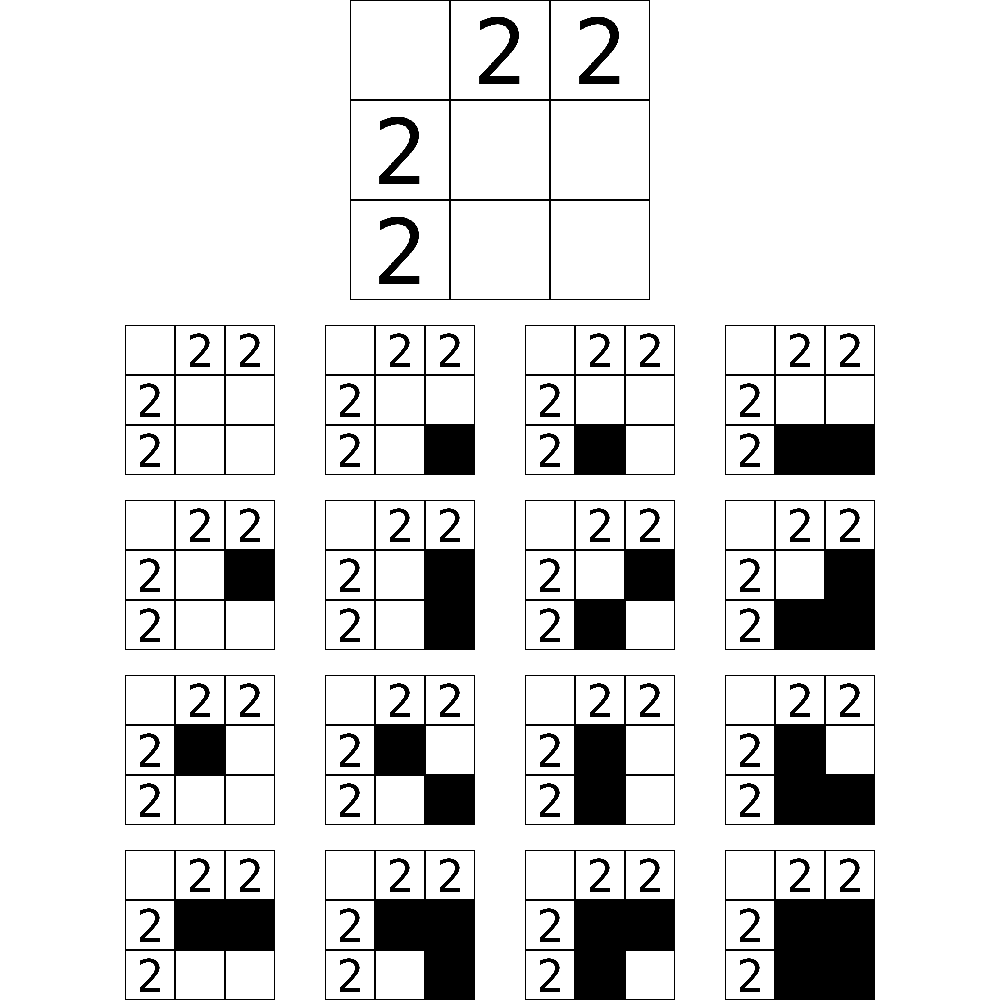
\includegraphics[width=0.5\textwidth]{images/all_solver_example.png}
    \caption{Solver całościowy sprawdza wszystkie możliwe układy planszy w celu znalezienia rozwiązania.}
\end{figure}

    Sposób działania tego solvera został przedstawiony w kodzie poniżej.

\begin{pseudokod}[H]
    %\SetAlTitleFnt{small}
    \SetArgSty{normalfont}
    \SetKwFunction{WeryfikujRozwiazanie}{WeryfikujRozwiazanie}
    \KwIn{Lista wierszy $R$, indeks pola $i$, lista wskazówek wierszy $Hr$ i kolumn $Hc$, szerokość $w$ i wysokość $h$ planszy}
    \KwOut{Czy znaleziono rozwiązanie \texttt{true/false}}
    \If{$i \geq w \cdot h$}{
        \texttt{return} \WeryfikujRozwiazanie{$R$, $Hr$, $Hc$, $w$, $h$}\;
    }
    \Else{
        $iWiersza \leftarrow \lceil \frac{i}{w} \rceil$\;
        $iKolumny \leftarrow i\ mod\ w$\;
        $R[iWiersza][iKolumny] \leftarrow 0$\;
        \If{\texttt{SolverCałościowy}($R, i+1, Hr, Hc, w, h$)}{
            \texttt{return true}\;
        }
        $R[iWiersza][iKolumny] \leftarrow 1$\;
        \texttt{return SolverCałościowy}($R, i+1, Hr, Hc, w, h$)\;
    }
    \caption{SolverCałościowy}\label{alg:allSolver}
\end{pseudokod}

    Solver ten zaczyna od pustej planszy. Następnie, dla pierwszego pola wywoływana jest rekursyjna
metoda: jeśli indeks pola mieści się w zakresie planszy, to najpierw jego status ustawiany jest na
pusty, i następuje wywołanie metody dla następnego indeksu, a jeśli rozwiązanie nie zostanie znalezione,
to pole jest wypełniane i ponownie dochodzi do wywołania metody na następnym polu. Jeśli indeks
wykracza poza zakres planszy, to znaczy, że wszystkie pola mają ustawiony status i wywoływana jest
metoda sprawdzająca poprawność rozwiązania, podobna do tej opisanej w \ref{alg:axisValidation}.
Jeśli solver zakończy działanie zwracając \texttt{true}, to w przekazanej mu macierzy pól 
(równoznaczne z listą wierszy) znajdzie się rozwiązanie łamigłówki.

    Ta wersja solvera cechuje się wysoką złożonością obliczeniową. Procedura sprawdzająca poprawność
rozwiązania zostanie wywołana $2^n$ razy w najgorszym przypadku, gdzie $n$ to ilość pól na planszy.
Oprócz tego, na każdym poziomie rekursji zostaje wykonany zestaw operacji, którego złożoność można
określić jako stałą. Zważywszy, że drzewo wywołań jest drzewem binarnym, a każdy poziom zostaje
wywołany 2 razy rzadziej niż poprzedni, daje to dodatkowe 
$\frac{2^n}{2} + \frac{2^n}{4} + \ldots + 1 = 2^n - 1$ operacji do wykonania. Przyjmując złożoność
$\mathcal{O}(n^2)$ procedury weryfikującej, daje to złożoność
$\mathcal{O}(2^n) \cdot \mathcal{O}(n^2) + \mathcal{O}(2^n) \cdot \mathcal{O}(1) = \mathcal{O}(2^n \cdot n^2)$
solvera dla najgorszego przypadku.


\subsection{Solver osiowy}
    W odróżnieniu od solvera całościowego, solver osiowy korzysta ze wskazówek przy szukaniu rozwiązań.
Opiera się on na fakcie, że każda linia (wiersz lub kolumna) może znajdować się w jednym z możliwych
stanów, których liczba nigdy nie dojdzie do $2^x$, gdzie $x$ jest długością linii. Sprawdzając
rozwiązanie w tym solverze, gwarantowana jest poprawność w jednej z osi, co dodatkowo znacząco skraca
czas szukania rozwiązania.

\begin{figure}[!htb]
    \centering
    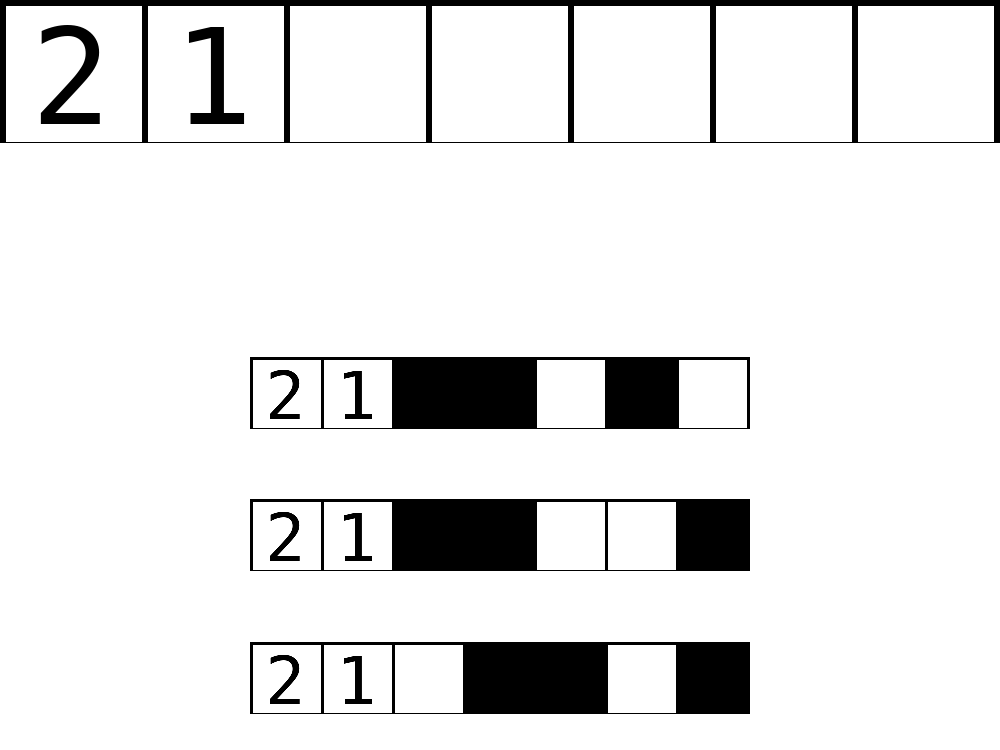
\includegraphics[width=0.5\textwidth]{images/axis_solver_example.png}
    \caption{Dla linii na grafice solver osiowy spradza jedynie 3 stany. Dla tej samej linii
solver całościowy sprawdziłby $2^5 = 32$ stany
    }
\end{figure}

    Zarys algorytmu w tej wersji został przedstawiony w kodzie.

\begin{pseudokod}[H]
    %\SetAlTitleFnt{small}
    \SetArgSty{normalfont}
    \SetKwFunction{WeryfikujRozwiazanie}{WeryfikujRozwiazanie}
    \SetKwFunction{NalozKombinacje}{NalozKombinacje}
    \KwIn{Lista linii $L$, indeks linii $i$, lista wskazówek linii prostopadłych $H$, ilość linii $n$}
    \KwOut{Czy znaleziono rozwiązanie \texttt{true/false}}
    \If{$i = n$}{
        \texttt{return} \WeryfikujRozwiazanie{$L$, $H$, $n$}\;
    }
    \Else{
        $linia \leftarrow L[i]$\;
        \ForEach{$komb \in linia.kombinacje$}{
            \NalozKombinacje{$linia, komb$}\;
            \If{\texttt{SolverOsiowy}($L, i+1, H, n$)}{
                \texttt{return true}\;
            }
        }
        \texttt{return false}\;
    }
    \caption{SolverOsiowy}\label{alg:axisSolver}
\end{pseudokod}

    Solver zaczyna od pustej planszy. Przed rozpoczęciem rozwiązywania sprawdzana jest ilość wszystkich
kombinacji w danej osi (iloczyn możliwości każdej z linii) i wybierana jest oś z mniejszą liczbą
możliwości. Następnie generowane są kombinacje dla każdej z linii. Solver korzysta z rekursyjnej
metody i ustawia pierwszą kombinację dla pierwszej linii. Następnie wywołuje metodę dla kolejnej linii,
aż do ostatniej, i wtedy weryfikuje rozwiązanie. Jeśli dla danego ustawienia w linii łamigłówka
nie ma rozwiązania, to solver przechodzi do kolejnego ustawienia i wywołuje metodę w kolejnej linii.

    Dzięki eliminacji kombinacji sprzecznych ze wskazówkami w danej osi, procedura sprawdzania
poprawności rozwiązania jest wywoływana o wiele rzadziej niż w przypadku solvera całościowego.
O ile ilość kombinacji w linii przy rozpatrywaniu każdej komórki z osobna to $2^n$, gdzie $n$ to
długość linii, tak w przypadku rozważania poprawnych kombinacji dla linii jest ona zależna od
długości i zawartości wskazówki, i można ją ograniczyć z góry przez
${n + 1 - h} \choose h$, a $h$ to ilość liczb we wskazówce dla danej linii. 
To przybliżenie jest zawyżone, ponieważ
zakłada występowanie jedynie bloków długości jeden we wskazówce. W przeciętnym przypadku, bloki
wypełnionych komórek będą dłuższe, oraz będzie ich mniej. Co więcej, jak zostało wspomniane na początku,
weryfikacja jest wymagana jedynie w jednej z dwóch osi, jako że konstrukcja potencjalnych rozwiązań
opiera się o zestawianie poprawnych kombinacji z linii.


\subsection{Solver eliminacyjny}
    Solverem, którego wariant znajduje się w aplikacji, jest solver eliminacyjny. W przeciwieństwie
do wcześniej opisanych solverów, solver ten nie zakłada układów komórek w liniach tak długo, jak to
możliwe. W przypadku tego solvera, generowane są możliwe kombinacje dla każdej z linii (zarówno wierszy, jak i
kolumn). W danym przejściu eliminowane są kombinacje sprzeczne z dostępnymi informacjami 
(np. kombinacje posiadające pełną pierwszą komórkę, podczas gdy pewne jest, że jest ona pełna) 
oraz wyciągane są części wspólne kombinacji (np. wszystkie kombinacje mają pustą drugą komórkę), 
które dostarczają informacji dla innych linii. Co więcej, w przeciwieństwie do poprzednich solverów,
nie jest konieczna walidacja rozwiązania, jako że rozwiązanie jest poprawne w momencie, gdy każdy
wiersz i każda kolumna ma dostępną jedną możliwą kombinację.

\begin{figure}[!htb]
    \centering
    \begin{subfigure}[b]{0.35\textwidth}
        \centering
        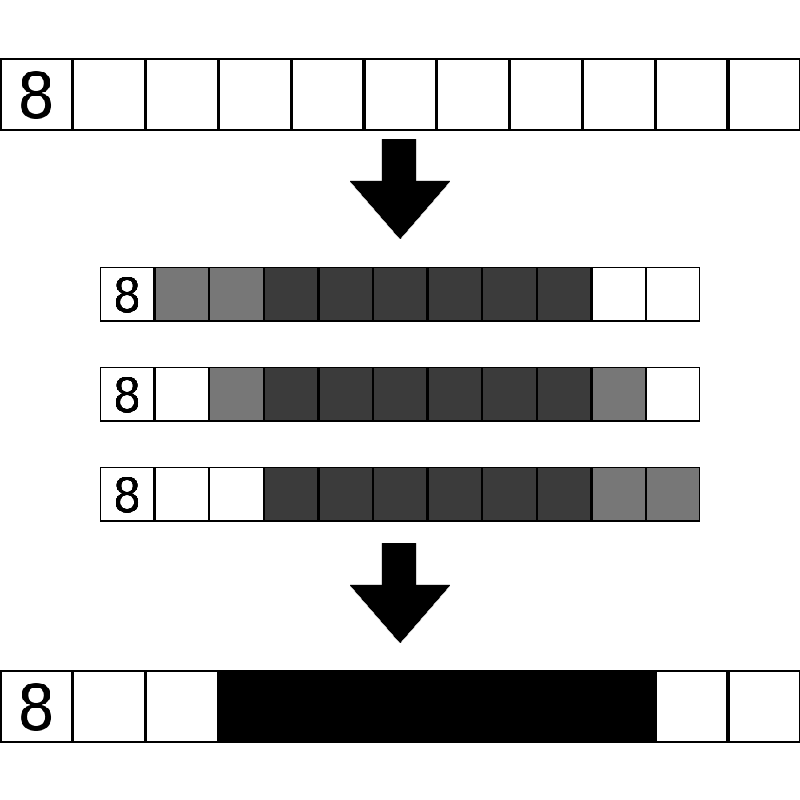
\includegraphics[width=\textwidth]{images/elimination_solver_example_a.png}
        \caption{pola wspólne dla wszystkich kombinacji zostają naniesione na planszę}
    \end{subfigure}
    \hspace{0.1\textwidth}
    \begin{subfigure}[b]{0.35\textwidth}
        \centering
        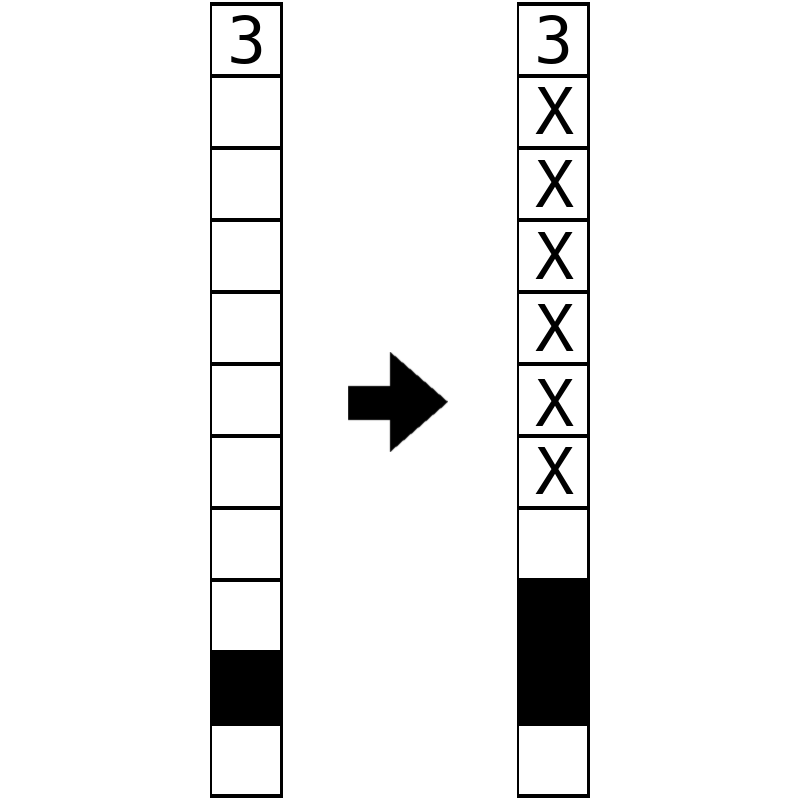
\includegraphics[width=\textwidth]{images/elimination_solver_example_b.png}
        \caption{korzystając z informacji z wiersza, solver wnioskuje stan większości pól w kolumnie
        (x oznacza pole definitywnie puste)}
    \end{subfigure}
    \caption{Przykład wnioskowania na podstawie możliwych kombinacji}
\end{figure}

    Główna procedura tego solvera oraz fragment odpowiedzialny za sprawdzanie danej linii zostały
przedstawione za pomocą pseudokodu.

\begin{pseudokod}[H]
    %\SetAlTitleFnt{small}
    \SetArgSty{normalfont}
    \SetKwFunction{SprawdzLinie}{SprawdzLinie}
    \SetKwFunction{NalozKombinacje}{NalozKombinacje}
    \SetKwFunction{UzupelnijKolejke}{UzupelnijKolejke}
    \KwIn{Lista wierszy $R$ i kolumn $C$, kolejka $Q$}
    \KwOut{Czy znaleziono rozwiązanie \texttt{true/false}}
    \While{$Q.zawieraElementy()$}{
        $linia \leftarrow Q.pop()$\;
        \SprawdzLinie{$linia$}\;
    }
    \If{$(\forall linia \in R \bigcup C)(|linia.kombinacje| = 1)$}{
        \texttt{return true}\;
    }
    \uElseIf{$(\exists linia \in R \bigcup C)(|linia.kombinacje| = 0)$}{
        \texttt{return false}\;
    }
    \Else{
        $zakladanaLinia \leftarrow$ pierwsza linia z wieloma kombinacjami\;
        \ForEach{$komb \in zakladanaLinia.kombinacje$}{
            $kopiaR \leftarrow kopiuj(R)$\;
            $kopiaC \leftarrow kopiuj(C)$\;
            \NalozKombinacje{$zakladanaLinia, komb$}\;
            \UzupelnijKolejke{$Q$}\;
            \If{\texttt{SolverEliminacyjny}($kopiaR, kopiaC, Q$)}{
                $R \leftarrow kopiaR$\;
                $C \leftarrow kopiaC$\;
                \texttt{return true}\;
            }
        }
        \texttt{return false}\;
    }
    \caption{SolverEliminacyjny}\label{alg:eliminationSolver}
\end{pseudokod}

\begin{pseudokod}[h]
    %\SetAlTitleFnt{small}
    \SetArgSty{normalfont}
    \SetKwFunction{WeryfikujKombinacje}{WeryfikujKombinacje}
    \KwIn{Linia $l$}
    \ForEach{$komb \in l.kombinacje$}{
        \If{\texttt{!WeryfikujKombinacje}($komb, l$)}{
            $l.kombinacje.usun(komb)$\;
        }
    }
    \ForEach{$i \in \{1, 2, \ldots, |l|\}$}{
        \If{$l[i] =$ \textit{nieznany} $\land$ pole identyczne we wszystkich kombinacjach}{
            $l[i] = $ nowy stan\;
            $Q.dodaj$(linia prostopadła do $l$ o indeksie $i$)\;
        }
    }
    \caption{SprawdzLinie}\label{alg:eliminationSolver_checkLine}
\end{pseudokod}

    Solver zaczyna od pustej planszy. Na początku generowane są wszystkie kombinacje dla każdej z
linii, a linie wrzucane są do kolejki \textit{last-in first-out}. Następnie solver przechodzi do
rozwiązywania. Dopóki kolejka nie jest pusta, to są linie, których kombinacje należy zweryfikować.
Z kolejki usuwana jest sprawdzana linia. Dla tej linii następują dwa kroki: najpierw, eliminowane
są kombinacje sprzeczne z układem danej linii. W wypadku tego solvera, każda komórka znajduje się
w jednym z trzech stanów: \textit{pełny}, \textit{pusty} i \textit{nieznany}. Stan \textit{nieznany}
komórki dopuszcza kombinacje zawierające komórkę pełną lub pustą; pozostałe stany wymagają
zgodności stanu ze stanem komórki w kombinacji. Po eliminacji sprzecznych kombinacji, dochodzi
do porównania kombinacji. Jeśli istnieje komórka w linii, której stan jest \textit{nieznany}, a
wszystkie pozostałe kombinacje mają ustawiony dla niej ten sam stan, to stan komórki jest aktualizowany,
a prostopadła linia zostaje dodana do kolejki do weryfikacji (następuje przy tym upewnienie, że
w kolejce nie ma powtórzeń). Kiedy kolejka zostanie opróżniona, sprawdzane są linie.
Jeśli wszystkie linie mają jeden możliwy stan, to znaczy, że zostało znalezione rozwiązanie. Jeśli
któraś z linii nie ma możliwej kombinacji, to nie istnieje rozwiązanie przy dokonanych założeniach.
W przeciwnym wypadku, solver zakłada poprawność jednej z kombinacji dla linii
o kilku możliwych kombinacjach. Jako że wskutek założenia stan linii zmienił się, to do kolejki
dodawane są linie prostopadłe. Następnie wywoływana jest w sposób rekursyjny metoda rozwiązująca
nonogram dla obecnego stanu planszy. Jeśli rozwiązanie nie zostanie znalezione w tej gałęzi, to
solver zakłada poprawność kolejnej kombinacji dla tej linii.

    Istotna uwaga dotyczy charakterystyki wierszy i kolumn. W celu umożliwienia działania procedury
został wykorzystany mechanizm obecny w wielu powszechnie używanych językach programowania, mianowicie
mechanizm płytkiej kopii. Mimo że listy wierszy i kolumn zawierają inne obiekty (listy), to obiekty
komórek przechowywane w tych zagnieżdżonych listach są takie same. Dzięki temu, modyfikując stan
komórki w liście wierszy w $n$-tym wierszu i $m$-tej komórce, modyfikujemy także stan komórki
zawartej w $n$-tej komórce w $m$-tej kolumnie w liście kolumn.

    Zaproponowany solver jest dobrze przystosowany do rozwiązywania łamigłówek, dla których nie
następuje zakładanie układu dowolnej linii. W wypadku takich łamigłówek, solver ten wykonuje procedurę
\texttt{SprawdzLinie} pewną ilość razy, a następnie upewnia się, że każda linia ma jedną dostępną
kombinację. Wyliczenie kombinacji dla wszystkich linii wymaga dostępu do $w+h$ zmiennych, co oznacza $w+h$ operacji
wykonanych w stałym czasie. Ilość wykonań procedury \texttt{SprawdzLinie} można ograniczyć z góry
przez $w+h+n$, gdzie $n$ to ilość pól na planszy, ponieważ pierwsze $w+h$ wykonań jest narzucone 
przez zapełnienie kolejki wszystkimi liniami przed przystąpieniem do rozwiązywania, a każde kolejne
wykonanie jest skutkiem określenia stanu przynajmniej jednego z pól na planszy, jako że jest to 
jedyny sposób na dodanie linii do kolejki. Weryfikacja pojedynczej kombinacji jest wykonywana w
czasie wielomianowym, jednak ilość kombinacji nie jest wielomianowa: dla wskazówek wypełnionych
samymi jedynkami wynosi
${n + 1 - h} \choose h$, gdzie $h$ to ilość liczb we wskazówce. Gdyby jednak ograniczyć ilość
liczb we wskazówkach, to możliwa ilość kombinacji będzie wielomianowo zależna od wielkości planszy.
Zatem dla podklasy nonogramów, która składa się z łamigłówek możliwych do rozwiązania bez dokonywania
zakładania stanu jednej z linii, i w których długość wskazówki jest ograniczona, solver ten
uzyskuje złożoność wielomianową.



\section{Porównanie wydajności solverów}
    W tej części zbadane zostały wydajności poszczególnych wersji solverów oraz wpływ wybranych
modyfikacji i heurystyk na ich wydajność.

\subsection{Metodyka badań}\label{metodyka}

\subsubsection{Ogólna metodyka}
    Metoda prowadzenia badań jest następująca: dla każdej łamigłówki prowadzonych jest 5 prób 
rozwiązania. Próby z minimalnym oraz maksymalnym czasem rozwiązywania zostają odrzucone, w celu
eliminacji błędów powstałych na skutek zaburzeń występujących w trakcie prowadzenia testu. Następnie
czas pozostałych 3 prób zostaje uśredniony i podany jako wynik badania. Jeśli czas wykonania
iteracji testu przekroczy 5 minut, to test zostaje przerwany i do komórki zostaje wpisany wynik
\textit{przekroczono}.

\subsubsection{Środowisko}
    Testy zostały przeprowadzone w systemie Ubuntu 20.04.3 LTS w wersji 64-bitowej.
System został zainstalowany na komputerze z procesorem Intel Core i5-6300HQ, z dostępem do
16GB pamięci RAM o taktowaniu 2133Mhz. Testy zostały uruchomione w środowisku Node.js \cite{node}
w wersji v14.18.2. Czas rozwiązywania łamigłówek na urządzeniu mobilnym może znacząco odbiegać
od czasów zaprezentowanych w wynikach, z powodu mniejszych zasobów i zastosowanego środowiska
uruchomieniowego.

\subsubsection{Prezentacja wyników}
    Wyniki zostały zaprezentowane w tabelach o następującym układzie: w pierwszych dwóch kolumnach
zostały podane nazwy łamigłówek i ich wielkości (łamigłówki są zadane na planszach kwadratowych).
W kolejnych kolumnach, nazwanych odpowiednio do zastosowanej modyfikacji bądź jej braku,
podany jest czas rozwiązywania nonogramu wyrażony w milisekundach. Czas jest zaokrąglony do pełnych
milisekund, zatem dla prostych łamigłówek może być wyrażony jako 0.

\subsubsection{Zestaw danych}
    Zestaw danych użyty do testów został przedstawiony na końcu rozdziału.


\subsection{Solver całościowy}
    Wydajność solvera całościowego została sprawdzona na zestawie 4 łamigłówek.

\subsubsection{Wyniki}
\begin{table}[h!]
    \begin{center}
        \begin{tabular}{|c|c|r|}
            \hline
            Nazwa          & Rozmiar        & Czas rozwiązywania w ms \\
            \hline
            Cross       & 3 & 1                     \\
            Flame       & 5 & 46                    \\
            Jellyfish   & 8 & \textit{przekroczono} \\
            Candy       & 8 & \textit{przekroczono} \\
            \hline
        \end{tabular}
    \end{center}
    \caption{Wyniki testów dla solvera całościowego}
\end{table}

\subsubsection{Interpretacja}
    Solver całościowy jest w stanie dość szybko rozwiązać niewielkie łamigłówki,
ale czas jego pracy rośnie bardzo szybko wraz ze wzrostem wielkości planszy. Wynik taki jest oczekiwany,
ponieważ z każdym dodatkowym polem, solver średnio podwaja swój czas pracy. Przejście z łamigłówki
wielkości 5x5 na łamigłówkę 8x8 wiązałoby się zatem z około $2^{8 \cdot 8 - 5 \cdot 5}$-krotnym wydłużeniem
czasu pracy. Pomijając kwestię budowy samych łamigłówek, przyjmując 46 milisekund jako czas pracy 
dla łamigłówki wielkości 5, daje to około 800 lat pracy solvera dla łamigłówki wielkości 8.


\subsection{Solver osiowy}
    Wydajność solvera całościowego została sprawdzona na pełnym zestawie 18 łamigłówek. Został
on poddany jednej modyfikacji.

\subsubsection{Modyfikacje}
    \textbf{Częściowa weryfikacja} rozwiązania polega na wykorzystaniu procedury częściowej weryfikacji.
Jest ona podobna do procedury weryfikacji w osi, ale nie sprawdza poprawności całej planszy,
a jedynie sprawdza, czy dany układ może prowadzić do poprawnego rozwiązania (czyli czy nie ma sprzeczności na tym etapie).
Procedura otrzymuje głębokość, dla jakiej ma zweryfikować poprawność. Jeśli do danej głębokości nie
występuje sprzeczność, to rozwiązanie jest konstruowane dalej. W przeciwnym przypadku, w danej gałęzi
nie może być poprawnego rozwiązania, i solver przechodzi do innej gałęzi.

\begin{figure}[h]
    \centering
    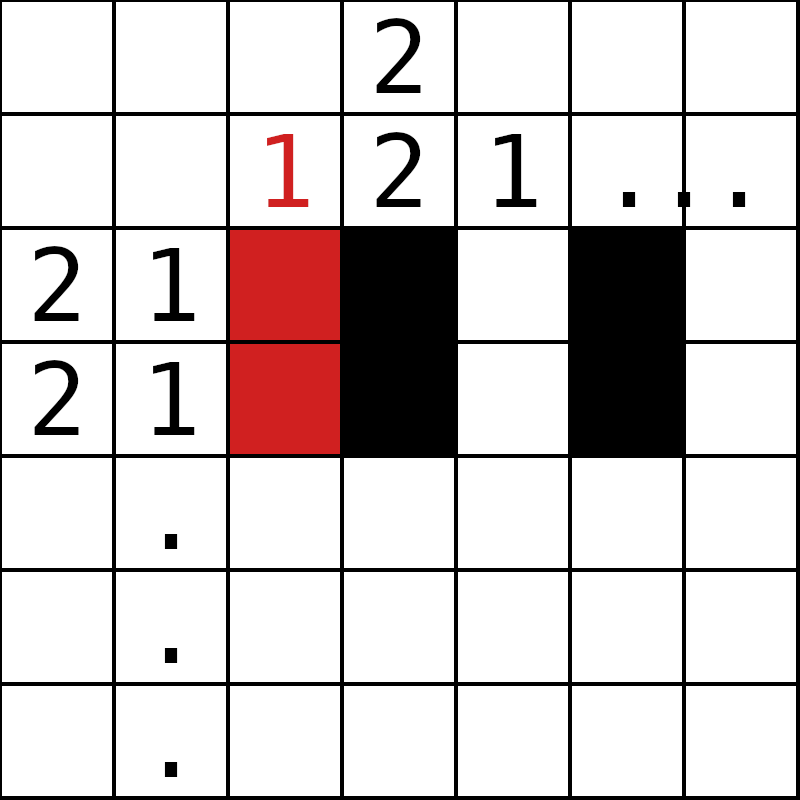
\includegraphics[width=0.4\textwidth]{images/partial_check_example.png}
    \caption{Na tym etapie można zdyskwalifikować każde rozwiązanie zawierające pierwszy i drugi wiersz
w układzie widocznym na grafice}
\end{figure}

\subsubsection{Wyniki}
\begin{table}[!htb]
    \begin{center}
        \begin{tabular}{|c|c|r r|}
            \hline
            {}          & {}        & \multicolumn{2}{c|}{Czas rozwiązywania w ms} \\
            Nazwa       & Rozmiar   & bez modyfikacji & z częściową weryfikacją \\
            \hline
            Cross       & 3         & 0                     & 0 \\
            Flame       & 5         & 0                     & 0 \\
            Jellyfish   & 8         & 463                   & 2 \\
            Candy       & 8         & 0                     & 0 \\
            Shield      & 10        & \textit{przekroczono} & 3 \\
            Dog         & 10        & 12004                 & 1 \\
            Duck        & 16        & \textit{przekroczono} & 12 \\
            Shrimp      & 16        & \textit{przekroczono} & 14 \\
            Cherries    & 20        & \textit{przekroczono} & 25 \\
            Potion      & 20        & \textit{przekroczono} & 315 \\
            Tape        & 25        & \textit{przekroczono} & 1091 \\
            Lighter     & 25        & \textit{przekroczono} & 60945 \\
            \hline
            Ghost       & 32        & \textit{przekroczono} & 40040 \\
            Demon       & 32        & \textit{przekroczono} & 3997 \\
            Butcher     & 48        & \textit{przekroczono} & \textit{przekroczono} \\
            Ranger      & 48        & \textit{przekroczono} & 59703 \\
            Orc         & 64        & \textit{przekroczono} & \textit{przekroczono} \\
            Swordsman   & 64        & \textit{przekroczono} & \textit{przekroczono} \\
            \hline
        \end{tabular}
    \end{center}
    \caption{Wyniki testów dla solvera osiowego}
\end{table}

\subsubsection{Interpretacja}
    W podstawowej wersji solver osiowy ma niewiele lepszą wydajność od solvera całościowego,
będąc w stanie rozwiązać niektóre łamigłówki wielkości 10 przy nałożonym ograniczeniu czasowym. 
Jednak po dodaniu częsciowej weryfikacji, wydajność solvera drastycznie wzrasta, i może zostać
wykorzystany do rozwiązywania łamigłówek o wiele większych niż w przypadku podstawowej wersji.
Pokazuje to, jak kluczowa jest wstępna eliminacja niepożądanych gałęzi przy rozwiązywaniu danego
problemu.


\subsection{Solver eliminacyjny}
    Wydajność solvera całościowego została sprawdzona na pełnym zestawie 18 łamigłówek.

\subsubsection{Modyfikacje}
    \textbf{Rozwiązywanie bez przerywania} (\textit{bez przerw.}) to modyfikacja polegająca na
usunięciu warunkowego przerwania szukania rozwiązania. Zamiast przerwać w momencie znalezienia
kolumny niezawierającej żadnej poprawnej kombinacji, solver szuka dalej, aż do opróżnienia kolejki,
i dopiero wtedy informuje o braku rozwiązania. Z uwagi na częste korzystanie z kolejki, eliminacja
tej instrukcji mogłaby skrócić czas wykonywania jednego sprawdzenia linii.

    \textbf{Zakładanie dla kolumn} (\textit{kolumny}) zmienia kolejność zakładania. Linia z wieloma
kombinacjami jest szukana najpierw na liście kolumn, a dopiero potem na liście wierszy. Ta modyfikacja
opiera się na założeniu, że układ wypełnionych pól w łamigłówkach może powodować lepszą wydajność
przy rozwiązywaniu z priorytetem dla osi pionowej.

    \textbf{Zakładanie dla linii z minimalną/maksymalną liczbą kombinacji} (\textit{min/max komb.})
dokonuje założenia dla linii z najmniejszą/największą liczbą poprawnych kombinacji. W ten sposób
badany jest wpływ doboru sposobu zakładania na czas szukania rozwiązania.

    \textbf{Kolejność linii w kolejce} to seria modyfikacji sprawdzających wpływ typu kolejki
na czas rozwiązania. W kolumnie \textit{lifo} podane są wyniki dla kolejki, w której nowo dodane
bądź ponownie dodane linie są przesuwane na początek kolejki. W \textit{fifo} przedmioty są wrzucane
na koniec kolejki. \textit{bez zm.} oznacza, że przedmioty są ustawiane na początku kolejki, ale
ponowne dodanie nie zmienia kolejności przedmiotów w kolejce. W kolejnych trzech kolumnach
(\textit{śl. ind. lifo}, \textit{śl. ind. fifo}, \textit{śl. ind. bez zm.}) badane są te same
własności kolejki, ale struktura ta zostaje zmodyfikowana tak, by śledzić linie wraz ze zmodyfikowanymi
indeksami. Dzięki temu nie jest konieczne sprawdzenie każdego indeksu w linii, a jedynie tych komórek,
dla których zaszła zmiana.


\subsubsection{Wyniki}

\begin{table}[h!]
    \begin{center}
        \begin{tabular}{|c|c|r r r r r|}
            \hline
            {}          & {}        & \multicolumn{5}{c|}{Czas rozwiązywania w ms} \\
            Nazwa       & Rozmiar   & bez modyfikacji & bez przerw. & kolumny & min komb. & max komb. \\
            \hline
            Cross       & 3         & 0     & 0     & 0     & 0     & 0     \\
            Flame       & 5         & 0     & 0     & 0     & 0     & 0     \\
            Jellyfish   & 8         & 1     & 1     & 1     & 1     & 1     \\
            Candy       & 8         & 0     & 0     & 0     & 0     & 0     \\
            Shield      & 10        & 2     & 2     & 2     & 2     & 1     \\
            Dog         & 10        & 1     & 0     & 0     & 0     & 1     \\
            Duck        & 16        & 2     & 1     & 1     & 1     & 1     \\
            Shrimp      & 16        & 1     & 1     & 1     & 1     & 1     \\
            Cherries    & 20        & 3     & 3     & 3     & 3     & 3     \\
            Potion      & 20        & 12    & 13    & 13    & 13    & 13    \\
            Tape        & 25        & 2     & 2     & 2     & 2     & 2     \\
            Lighter     & 25        & 13    & 13    & 13    & 12    & 13    \\
            \hline
            Ghost       & 32        & 47    & 47    & 48    & 45    & 47    \\
            Demon       & 32        & 1787  & 1817  & 1806  & 1800  & 1822  \\
            Butcher     & 48        & 1811  & 1809  & 1819  & 1790  & 1791  \\
            Ranger      & 48        & 46    & 48    & 47    & 47    & 48    \\
            Orc         & 64        & 1463  & 1454  & 1446  & 1465  & 1456  \\
            Swordsman   & 64        & 1440  & 1467  & 1451  & 1429  & 1432  \\
            \hline
        \end{tabular}
    \end{center}
    \caption{I część wyników dla solvera eliminacyjnego}
\end{table}

\begin{table}[h]
    \begin{center}
        \begin{tabular}{|c|c|r r r r r r|}
            \hline
            {}          & {}        & \multicolumn{6}{c|}{Czas rozwiązywania w ms} \\
            Nazwa       & Rozmiar   & lifo & fifo & bez zm. & śl. ind. lifo & śl. ind. fifo & śl. ind. bez zm. \\
            \hline
            Cross       & 3         & 0     & 0     & 0     & 0     & 0     & 0     \\
            Flame       & 5         & 0     & 0     & 0     & 0     & 0     & 0     \\
            Jellyfish   & 8         & 1     & 2     & 2     & 2     & 1     & 1     \\
            Candy       & 8         & 0     & 0     & 0     & 0     & 0     & 0     \\
            Shield      & 10        & 2     & 1     & 1     & 2     & 3     & 2     \\
            Dog         & 10        & 1     & 1     & 1     & 1     & 0     & 1     \\
            Duck        & 16        & 2     & 1     & 2     & 2     & 2     & 2     \\
            Shrimp      & 16        & 1     & 1     & 1     & 1     & 1     & 1     \\
            Cherries    & 20        & 3     & 4     & 4     & 3     & 4     & 3     \\
            Potion      & 20        & 12    & 13    & 14    & 16    & 16    & 13    \\
            Tape        & 25        & 2     & 2     & 2     & 4     & 3     & 3     \\
            Lighter     & 25        & 13    & 13    & 13    & 13    & 15    & 13    \\
            \hline
            Ghost       & 32        & 47    & 47    & 52    & 56    & 72    & 54    \\
            Demon       & 32        & 1787  & 2380  & 1980  & 1194  & 1257  & 1127  \\
            Butcher     & 48        & 1811  & 1884  & 1798  & 1854  & 1962  & 1717  \\
            Ranger      & 48        & 46    & 44    & 53    & 61    & 62    & 59    \\
            Orc         & 64        & 1463  & 1413  & 1437  & 1413  & 1415  & 1311  \\
            Swordsman   & 64        & 1440  & 1489  & 1544  & 1534  & 1608  & 1451  \\
            \hline
        \end{tabular}
    \end{center}
    \caption{II część wyników dla solvera eliminacyjnego}
\end{table}

\subsubsection{Interpretacja}
    Solver eliminacyjny jest najszybszym z zaprezentowanych solverów. Jest w stanie rozwiązać
nawet największe, 64x64 nonogramy w nałożonym ograniczeniu czasowym. Każdą ze sprawdzanych łamigłówek
rozwiązuje szybciej niż solver osiowy. Na szczególną uwagę zasługuje szybkość rozwiązania nonogramów
\textit{Ghost} i \textit{Ranger}. Dzięki oparciu się o informacje, które zostały wywnioskowane z poprzednio
rozpatrywanych linii, solver może rozwiązać nawet łamigłówki o dużych rozmiarach bez zakładania
poprawności kombinacji dowolnej linii, lub z minimalną jego ilością.

    Pierwsza seria modyfikacji nie miała dużego wpływu na czas rozwiązywania. Część modyfikacji z
drugiej serii okazała się mieć kluczowy wpływ na wydajność solvera przy rozwiązywaniu danej łamigłówki. Użycie kolejki
typu \textit{first-in first-out} z przerzucaniem na koniec przy aktualizacji linii znacznie spowolniło
czas rozwiązywania łamigłówki \textit{Demon} w przypadku bazowej wersji solvera,
a w przypadku wersji ze śledzeniem indeksów różnica była mniejsza, ale zauważalna.
Oprócz tego, modyfikacja struktury danych w celu śledzenia modyfikowanych indeksów
okazała się dobrym pomysłem, jako że solver korzystający z niej (\textit{śl. ind. bez zm.}) osiągnął
najlepsze czasy dla trudniejszych łamigłówek (np. \textit{Demon}, \textit{Butcher}), 
będąc nieznacznie wolniejszym dla łamigłówek prostszych (np. \textit{Ghost}, \textit{Ranger}).


\subsection{Wnioski}
    Złożoność solvera całościowego bardzo ogranicza jego przydatność w rozwiązywaniu nonogramów.
Solver osiowy, dzięki ograniczeniu ilości kombinacji dla danej linii, okazał się od niego lepszy,
ale tylko w niewielkim stopniu. Jednak poszerzenie solvera osiowego o częściową weryfikację rozwiązania
znacznie poprawiło jego osiągi. Solver eliminacyjny jest najwydajniejszym z zaproponowanych solverów. Dzięki oparciu na pewnych
informacjach i ograniczeniu zakładania, a co za tym idzie back-trackingu, może rozwiązać zadaną
łamigłówkę szybciej niż inne solvery.

    Przeprowadzane badania potwierdzają układ hierarchii solverów: solver osiowy osiąga lepsze wyniki
od solvera całościowego dzięki ograniczeniu się do zakładania w jednej osi. Najlepszym okazał
się solver eliminacyjny, który w miarę możliwości wyklucza zakładanie poprawności kombinacji.


\subsection{Zestaw danych}
    Do przeprowadzenia badań zostały użyte następujące obrazy, które po konwersji zostały przekazane do solverów
jako zestaw wskazówek. Grafiki zawierające kolor biały zostały nałożone na tło w kolorze magenta
w celu wyróżnienia tego koloru na tle białej kartki.

\begin{figure}[!htb]
    \centering
    \begin{subfigure}[b]{0.1\textwidth}
        \centering
        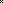
\includegraphics[width=\textwidth]{images/data_set/3x3_cross.png}
        \caption{Cross}
    \end{subfigure}
    \begin{subfigure}[b]{0.1\textwidth}
        \centering
        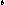
\includegraphics[width=\textwidth]{images/data_set/5x5_flame.png}
        \caption{Flame}
    \end{subfigure}
    \begin{subfigure}[b]{0.1\textwidth}
        \centering
        
\includegraphics[width=\textwidth]{images/data_set/8x8_jellyfish.png}
        \caption{Jellyfish \cite{8x8-src}}
    \end{subfigure}
    \begin{subfigure}[b]{0.1\textwidth}
        \centering
        
\includegraphics[width=\textwidth]{images/data_set/8x8_candy.png}
        \caption{Candy \cite{8x8-src}}
    \end{subfigure}
    \begin{subfigure}[b]{0.1\textwidth}
        \centering
        
\includegraphics[width=\textwidth]{images/data_set/10x10_shield.png}
        \caption{Shield \cite{10x10-src}}
    \end{subfigure}
    \begin{subfigure}[b]{0.1\textwidth}
        \centering
        
\includegraphics[width=\textwidth]{images/data_set/10x10_dog.png}
        \caption{Dog \cite{10x10-src}}
    \end{subfigure}
    \begin{subfigure}[b]{0.1\textwidth}
        \centering
        
\includegraphics[width=\textwidth]{images/data_set/16x16_duck.png}
        \caption{Duck \cite{16x16-src_duck}}
    \end{subfigure}
    \begin{subfigure}[b]{0.1\textwidth}
        \centering
        
\includegraphics[width=\textwidth]{images/data_set/16x16_shrimp.png}
        \caption{Shrimp \cite{16x16-src_shrimp}}
    \end{subfigure}
    \begin{subfigure}[b]{0.1\textwidth}
        \centering
        
\includegraphics[width=\textwidth]{images/data_set/20x20_cherries.png}
        \caption{Cherries \cite{20x20-src}}
    \end{subfigure}
    \begin{subfigure}[b]{0.1\textwidth}
        \centering
        
\includegraphics[width=\textwidth]{images/data_set/20x20_potion.png}
        \caption{Potion \cite{20x20-src}}
    \end{subfigure}
    \begin{subfigure}[b]{0.1\textwidth}
        \centering
        
\includegraphics[width=\textwidth]{images/data_set/25x25_tape.png}
        \caption{Tape \cite{25x25-src}}
    \end{subfigure}
    \begin{subfigure}[b]{0.1\textwidth}
        \centering
        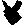
\includegraphics[width=\textwidth]{images/data_set/25x25_lighter.png}
        \caption{Lighter \cite{25x25-src}}
    \end{subfigure}
    \begin{subfigure}[b]{0.2\textwidth}
        \centering
        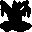
\includegraphics[width=\textwidth]{images/data_set/32x32_ghost.png}
        \caption{Ghost \cite{32x32-src}}
    \end{subfigure}
    \begin{subfigure}[b]{0.2\textwidth}
        \centering
        
\includegraphics[width=\textwidth]{images/data_set/32x32_demon.png}
        \caption{Demon \cite{32x32-src}}
    \end{subfigure}
    \begin{subfigure}[b]{0.2\textwidth}
        \centering
        
\includegraphics[width=\textwidth]{images/data_set/48x48_butcher.png}
        \caption{Butcher \cite{48x48-src_butcher}}
    \end{subfigure}
    \begin{subfigure}[b]{0.2\textwidth}
        \centering
        
\includegraphics[width=\textwidth]{images/data_set/48x48_ranger.png}
        \caption{Ranger \cite{48x48-src_ranger}}
    \end{subfigure}
    \begin{subfigure}[b]{0.4\textwidth}
        \centering
        
\includegraphics[width=\textwidth]{images/data_set/64x64_orc.png}
        \caption{Orc \cite{64x64-src_orc}}
    \end{subfigure}
    \begin{subfigure}[b]{0.4\textwidth}
        \centering
        
\includegraphics[width=\textwidth]{images/data_set/64x64_swordsman.png}
        \caption{Swordsman \cite{64x64-src_swordsman}}
    \end{subfigure}
    \caption{Zestaw danych}
\end{figure}



\section{Predefiniowane łamigłówki}


\subsection{Wymagania dla łamigłówek}
    Łamigłówki, które zostały umieszczone w aplikacji dla użytkownika, muszą spełniać pewne wymagania.

\subsubsection{Łamigłówka ma jedno rozwiązanie}
    Wynika to ze sposobu zapisu łamigłówki w aplikacji. Każda łamigłówka jest pewnym obrazkiem,
zapisanym w formie siatki komórek, które są puste lub odpowiednio zakolorowane. Gdyby dopuścić
łamigłówkę, która ma wiele rozwiązań, to każde rozwiązanie poza przewidzianym nie byłoby dopuszczane,
mimo jego poprawności.

\begin{figure}[!htb]
    \centering
    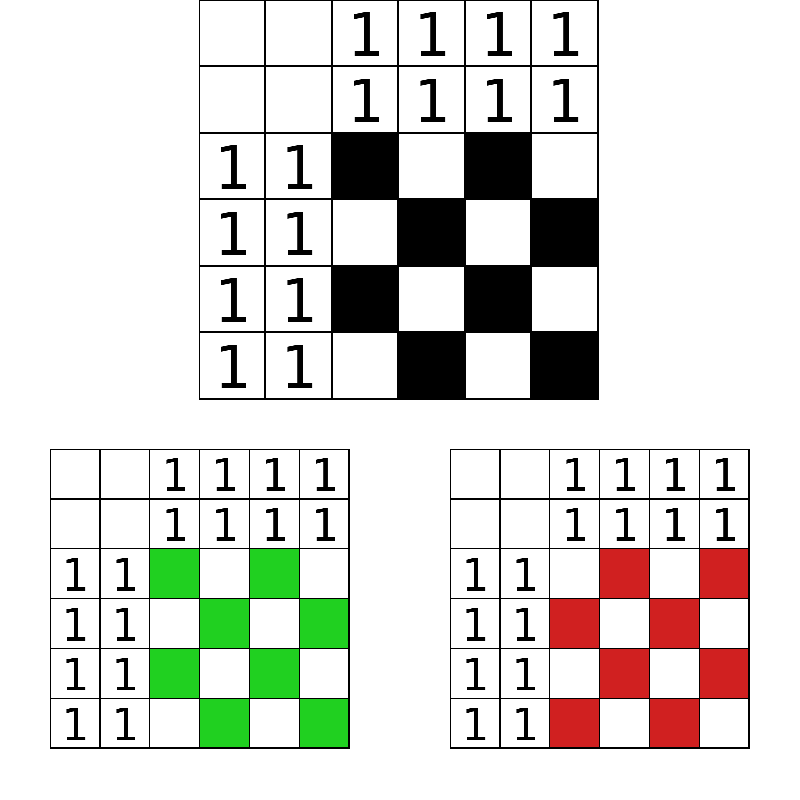
\includegraphics[width=0.6\textwidth]{images/no_unique_solution.png}
    \caption{Łamigłówka zdefiniowana na górze ma 2 rozwiązania, z których tylko jedno pokrywa się
z przewidzianym. Jeśli użytkownik zacznie rozwiązywać nonogram zakładając poprawność prawej wersji,
to aplikacja w nieuzasadniony sposób uzna to za błąd.}
\end{figure}

\subsubsection{Łamigłówka nie wymaga zakładania}
    Łamigłówki wymagające założenia poprawności jednego z wariantów na pewnym etapie są zdecydowanie
bardziej złożone od łamigłówek, które da się ułożyć zbierając informacje z pojedynczych wierszy i kolumn.
W przypadku solvera, założenie poprawności niewłaściwej kombinacji wymaga jedynie dokonania back-trackingu
i sprawdzenia kolejnej kombinacji. Użytkownik musi rozwiązać taką łamigłówkę w pamięci, ponieważ
zaznaczenie błędnej komórki na planszy wiązałoby się z wychwyceniem błędu przez aplikację.


\subsection{Zatwierdzenie spełniania wymienionych wymagań przez łamigłówkę}
    Do weryfikacji łamigłówki użyty został zmodyfikowany solver eliminacyjny. Brak konieczności
zakładania przy rozwiązywaniu łamigłówki został sprawdzony przez nakazanie solverowi rozwiązania
łamigłówki. Modyfikacja solvera polega na tym, że solver odrzuca łamigłówkę, jeśli kolejka linii do
sprawdzenia została opróżniona, ale łamigłówka nie została rozwiązana. Jeśli łamigłówka nie została
rozwiązana na tym etapie, to solver przejdzie do założeń: dla linii z wieloma poprawnymi
kombinacjami zakładałby poprawność jednej z nich. Jest to jednak sprzeczne z wymaganiem.

    Tak zmodyfikowany solver weryfikuje jednocześnie pierwsze kryterium. Znalezienie rozwiązania
łamigłówki bez dokonania założeń oznacza istnienie wyłącznie jednego rozwiązania. Wynika to z faktu,
że solver rozwiązuje łamigłówkę dokonując serii wnioskowań na liniach. W każdym wnioskowaniu solver
uzupełnia jedynie te pola, co do których stanu jest pewien. Rozwiązanie całej łamigłówki w ten sposób
oznacza, że każda komórka znajduje się w jedynym możliwym dla siebie stanie, co wyklucza istnienie
innych rozwiązań.
